
\section{講義概要}


\begin{frame}
\frametitle{今日の内容}



\begin{enumerate}
\item 原始関数, 不定積分
\item 部分積分, 置換積分
\item 部分分数分解, 有理関数の積分
\end{enumerate} 



\end{frame}




%%%%%%%%%%%%%%%%%%%%%%%%%%%%%%%%%%%%%%%%%%%%%%%%%%%%%%%%%%%%%%%%%%%%%%%%%%%%%%%%%%%%%%%
%%%%%%%%%%%%%%%%%%%%%%%%%%%%%%%%%%%%%%%%%%%%%%%%%%%%%%%%%%%%%%%%%%%%%%%%%%%%%%%%%%%%%%%



%%%%%%%%%%%%%%%%%%%%%%%%%%%%%%%%%%%%%%%%%%%%%%%%%%%%%%%%%%%%%%%%%%%%%%%%%%%%%%%%%%%%%%%
%%%%%%%%%%%%%%%%%%%%%%%%%%%%%%%%%%%%%%%%%%%%%%%%%%%%%%%%%%%%%%%%%%%%%%%%%%%%%%%%%%%%%%

\section{不定積分}


\begin{frame}
\frametitle{不定積分}

関数の微分に対する逆の演算を考える. 

\begin{Def}
関数$f(x)$, $F(x)$が開区間$I$で定義され, 
$$
F'(x) = f(x)
$$
を満たすとき, 関数$F(x)$を$f(x)$の\underline{原始関数}という. 
\end{Def}


\begin{itemize}
\item $x^2$と$x^2+5$は共に$2x$の原始関数. 
\item $e^x$と$e^x+3$は共に$e^x$の原始関数. 
\item $\sin x$と $\sin x-2$は共に$\cos x$の原始関数. 
\end{itemize}

\end{frame}

%%%%%%%%%%%%%%%%%%%%%%%%%%%%%%%%%%%%%%%%%%%%%%%%%%%%%%%%%%%%%%%%%%%%%%%%%%%%%%%%%%%%%%%
%%%%%%%%%%%%%%%%%%%%%%%%%%%%%%%%%%%%%%%%%%%%%%%%%%%%%%%%%%%%%%%%%%%%%%%%%%%%%%%%%%%%%%



\begin{frame}
\frametitle{不定積分}

与えられた関数$f(x)$の原始関数は定数差を除いて一意に決まる. 
実際, $F(x), G(x)$を$f(x)$の原始関数とすれば
$$
(F(x)-G(x))'=F'(x)-G'(x)=f(x)-f(x)=0
$$
であるから, 導関数が$0$となる関数が定数関数に限ることを示せば良い. 
(定数関数の導関数が$0$であることはすぐ分かるが, 逆は定義から自明ではない.)\\
\ \\

実際, $H'(x)=0$とすれば, 平均値の定理より任意の$a<b$に関して$c \in (a,b)$が存在して
$$
H(b)-H(a)=H'(c)(b-a)=0. 
$$

\end{frame}



%%%%%%%%%%%%%%%%%%%%%%%%%%%%%%%%%%%%%%%%%%%%%%%%%%%%%%%%%%%%%%%%%%%%%%%%%%%%%%%%%%%%%%%
%%%%%%%%%%%%%%%%%%%%%%%%%%%%%%%%%%%%%%%%%%%%%%%%%%%%%%%%%%%%%%%%%%%%%%%%%%%%%%%%%%%%%%



\begin{frame}
\frametitle{不定積分}


\begin{Def}
関数$f(x)$の原始関数の全体を\underline{不定積分}と呼び, 原始関数$F(x)$を用いて   
$$
\int f(x)dx = F(x)+C
$$
と表す. $C$は\underline{積分定数}と呼ばれ, 原始関数が定数差を除いて定まることを表す. 
また$f(x)$の不定積分を求めることを\underline{積分}するといい, $f(x)$は\underline{被積分関数}と呼ばれる.  
\end{Def}
 


\end{frame}





%%%%%%%%%%%%%%%%%%%%%%%%%%%%%%%%%%%%%%%%%%%%%%%%%%%%%%%%%%%%%%%%%%%%%%%%%%%%%%%%%%%%%%%
%%%%%%%%%%%%%%%%%%%%%%%%%%%%%%%%%%%%%%%%%%%%%%%%%%%%%%%%%%%%%%%%%%%%%%%%%%%%%%%%%%%%%%



\begin{frame}
\frametitle{不定積分}

不定積分は微分の逆操作であるから, 
\begin{itemize}
\item $\alpha \ne 1$に対して, $\displaystyle \int x^\alpha dx = \frac{1}{\alpha+1}x^{\alpha+1}+C$,
\item $\displaystyle \int \frac{1}{x}dx = \log |x|+C$,
\item $\displaystyle \int \sin x dx = -\cos x+C$, $\displaystyle \int \cos x dx = \sin x+C$
\end{itemize}
などが成立する. 

\end{frame}




%%%%%%%%%%%%%%%%%%%%%%%%%%%%%%%%%%%%%%%%%%%%%%%%%%%%%%%%%%%%%%%%%%%%%%%%%%%%%%%%%%%%%%%
%%%%%%%%%%%%%%%%%%%%%%%%%%%%%%%%%%%%%%%%%%%%%%%%%%%%%%%%%%%%%%%%%%%%%%%%%%%%%%%%%%%%%%



\begin{frame}
\frametitle{積分定数に関する注意}

積分定数に関して注意をしておく. \\
\ \\

関数$\frac{1}{x}$の定義域は$(-\infty,0)$と$(0,\infty)$の和集合であるから, 厳密には定数$C_1,C_2$を用いて
\begin{itemize}
\item $(x>0): \ \int \frac{1}{x}dx = \log x + C_1$
\item $(x<0): \ \int \frac{1}{x}dx = \log (-x) + C_2$
\end{itemize}
と書かれるべきであるが, これを暗黙の了解として
$$
 \int \frac{1}{x}dx = \log |x| +C
$$
と書く. (原始関数の差は局所定数関数というのが正しい.)\\
\ \\

記号の簡略化のために, 積分定数はしばしば省略される. この講義でも以下では省略する.  

\end{frame}


%%%%%%%%%%%%%%%%%%%%%%%%%%%%%%%%%%%%%%%%%%%%%%%%%%%%%%%%%%%%%%%%%%%%%%%%%%%%%%%%%%%%%%%
%%%%%%%%%%%%%%%%%%%%%%%%%%%%%%%%%%%%%%%%%%%%%%%%%%%%%%%%%%%%%%%%%%%%%%%%%%%%%%%%%%%%%%



\begin{frame}
\frametitle{不定積分の性質}

和・差や定数倍の微分は, 微分の和・差や定数倍となった. 
積分に関しても同様である.  
微分と積分のこの性質は線形性と呼ばれる. 

\begin{Thm}
$\alpha, \beta \in \R$に対して
\begin{align*}
\int (\alpha f(x) + \beta g(x))dx = \alpha \int f(x)dx + \beta \int g(x) dx.  
\end{align*}
\end{Thm}

例えば, 
\begin{align*}
\int (4x^3-5x)dx &= 4 \int x^3dx - 5 \int xdx = x^4-\frac{5}{2}x^2, \\
\int (\sin x - 2e^x) dx & = \int \sin x dx - 2 \int e^x dx = -\cos x -2e^x. 
\end{align*}

\end{frame}



%%%%%%%%%%%%%%%%%%%%%%%%%%%%%%%%%%%%%%%%%%%%%%%%%%%%%%%%%%%%%%%%%%%%%%%%%%%%%%%%%%%%%%%
%%%%%%%%%%%%%%%%%%%%%%%%%%%%%%%%%%%%%%%%%%%%%%%%%%%%%%%%%%%%%%%%%%%%%%%%%%%%%%%%%%%%%%


\section{部分積分}

\begin{frame}
\frametitle{部分積分の公式}

微分と積分は互いに逆の演算であるから, 微分に関する公式は積分の公式に書き直すことができる. 

\begin{Thm}[部分積分の公式]
$$
\int f(x)g'(x)dx = f(x)g(x) - \int f'(x)g(x)dx
$$
\end{Thm}

実際, 積の微分法より
$$
(f(x)g(x))'=f'(x)g(x)+f(x)g'(x). 
$$
両辺を積分すると
$$
f(x)g(x)=\int f'(x)g(x)dx +\int f(x)g'(x)dx.
$$


\end{frame}


%%%%%%%%%%%%%%%%%%%%%%%%%%%%%%%%%%%%%%%%%%%%%%%%%%%%%%%%%%%%%%%%%%%%%%%%%%%%%%%%%%%%%%%
%%%%%%%%%%%%%%%%%%%%%%%%%%%%%%%%%%%%%%%%%%%%%%%%%%%%%%%%%%%%%%%%%%%%%%%%%%%%%%%%%%%%%%



\begin{frame}
\frametitle{部分積分の公式}

部分積分の公式
$$
\int f(x)g'(x)dx = f(x)g(x) - \int f'(x)g(x)dx
$$
を用いて$\int x e^x dx$を計算する. 
\begin{align*}
\int x e^x dx &= \int x(e^x)'dx \\
& = xe^x-\int(x)'e^xdx \\
&= xe^x-\int e^xdx \\
& = xe^x - e^x. 
\end{align*}
実際, 
$$
(xe^x - e^x)'=e^x+xe^x-e^x=xe^x. 
$$

\end{frame}




%%%%%%%%%%%%%%%%%%%%%%%%%%%%%%%%%%%%%%%%%%%%%%%%%%%%%%%%%%%%%%%%%%%%%%%%%%%%%%%%%%%%%%%
%%%%%%%%%%%%%%%%%%%%%%%%%%%%%%%%%%%%%%%%%%%%%%%%%%%%%%%%%%%%%%%%%%%%%%%%%%%%%%%%%%%%%%



\begin{frame}
\frametitle{部分積分の公式}

\begin{align*}
\int \log x dx & = \int (x)'\log x dx \\
& = x \log x -\int x(\log x)'dx \\
&= x \log x - \int 1 dx \\
& = x\log x -x.  
\end{align*}
実際, 
$$
(x\log x -x)' = \log x + x \cdot \frac{1}{x}-1=\log x. 
$$


\end{frame}


%%%%%%%%%%%%%%%%%%%%%%%%%%%%%%%%%%%%%%%%%%%%%%%%%%%%%%%%%%%%%%%%%%%%%%%%%%%%%%%%%%%%%%%
%%%%%%%%%%%%%%%%%%%%%%%%%%%%%%%%%%%%%%%%%%%%%%%%%%%%%%%%%%%%%%%%%%%%%%%%%%%%%%%%%%%%%%



\begin{frame}
\frametitle{部分積分の公式}

\begin{align*}
\int x \cos x dx & = \int x(\sin x)' dx\\
& = x \sin x - \int (x)' \sin x dx \\
& = x \sin x - \int \sin x dx \\
&= x \sin x + \cos x. 
\end{align*}
実際,
$$
(x \sin x + \cos x)' = \sin x + x \cos x -\sin x=x \cos x. 
$$

\end{frame}


%%%%%%%%%%%%%%%%%%%%%%%%%%%%%%%%%%%%%%%%%%%%%%%%%%%%%%%%%%%%%%%%%%%%%%%%%%%%%%%%%%%%%%%
%%%%%%%%%%%%%%%%%%%%%%%%%%%%%%%%%%%%%%%%%%%%%%%%%%%%%%%%%%%%%%%%%%%%%%%%%%%%%%%%%%%%%%



\begin{frame}
\frametitle{部分積分の公式}

\begin{Prob}
次の不定積分を計算せよ. 
\begin{enumerate}
\item $\int (3x+1)e^{x}dx$
\item $\int x \log x dx$
\item $\int x^2 \sin x dx$
\end{enumerate}
\end{Prob}

\end{frame}



%%%%%%%%%%%%%%%%%%%%%%%%%%%%%%%%%%%%%%%%%%%%%%%%%%%%%%%%%%%%%%%%%%%%%%%%%%%%%%%%%%%%%%%
%%%%%%%%%%%%%%%%%%%%%%%%%%%%%%%%%%%%%%%%%%%%%%%%%%%%%%%%%%%%%%%%%%%%%%%%%%%%%%%%%%%%%%



\begin{frame}
\frametitle{部分積分の公式}


\begin{align*}
\int (3x+1)e^{x}dx & = \int (3x+1) (e^{x})'dx = (3x+1)e^x -\int 3 e^x dx \\
& = (3x+1)e^x-3e^x=(3x-2)e^x
\end{align*}
\begin{align*}
\int x \log x dx & = \int (\frac{1}{2}x^2)'\log x dx = \frac{1}{2}x^2 \log x - \int \frac{1}{2}x^2 \cdot \frac{1}{x}dx \\
& =  \frac{1}{2}x^2 \log x -\frac{1}{4}x^2
\end{align*}
\begin{align*}
\int x^2 \sin x dx & = \int x^2(-\cos x)'dx = x^2(-\cos x) + \int 2x \cos x dx \\
& = -x^2 \cos x +2(x\sin x + \cos x)
\end{align*}


\end{frame}


%%%%%%%%%%%%%%%%%%%%%%%%%%%%%%%%%%%%%%%%%%%%%%%%%%%%%%%%%%%%%%%%%%%%%%%%%%%%%%%%%%%%%%%
%%%%%%%%%%%%%%%%%%%%%%%%%%%%%%%%%%%%%%%%%%%%%%%%%%%%%%%%%%%%%%%%%%%%%%%%%%%%%%%%%%%%%%

\section{置換積分}

\begin{frame}
\frametitle{置換積分}

\begin{Thm}[置換積分の公式] \label{置換積分の公式}
関数$f(x)$の変数$x$が別の変数$t$の$C^1$級関数$x=\phi(t)$として表されるとき
$$
\int f(x)dx =\int f(\phi(t))\phi'(t)dt
$$
ここで左辺$\int f(x)dx$は$t$の関数と考えている. 
\end{Thm}
\begin{itemize}
\item 置換積分の公式は積分する変数を$x$から$t$に変換するための公式. 
\item  微分記号$\phi'(t)=\frac{dx}{dt}$を分数のように扱って
 $$
 \frac{dx}{dt} dt = dx
 $$
 と考えることができる. 
 \end{itemize}
\end{frame}



%%%%%%%%%%%%%%%%%%%%%%%%%%%%%%%%%%%%%%%%%%%%%%%%%%%%%%%%%%%%%%%%%%%%%%%%%%%%%%%%%%%%%%%
%%%%%%%%%%%%%%%%%%%%%%%%%%%%%%%%%%%%%%%%%%%%%%%%%%%%%%%%%%%%%%%%%%%%%%%%%%%%%%%%%%%%%%



\begin{frame}
\frametitle{定理\ref{置換積分の公式}の証明}

$F(x)=\int f(x)dx$とすれば, 合成関数の微分法より
$$
(F(\phi(t)))'=F'(\phi(t))\phi'(t)=f(\phi(t))\phi'(t). 
$$
これを$t$で積分して
$$
F(\phi(t))= \int f(\phi(t))\phi'(t)dt. 
$$
このように置換積分は合成関数の微分法の逆操作といえる. 

\end{frame}




%%%%%%%%%%%%%%%%%%%%%%%%%%%%%%%%%%%%%%%%%%%%%%%%%%%%%%%%%%%%%%%%%%%%%%%%%%%%%%%%%%%%%%%
%%%%%%%%%%%%%%%%%%%%%%%%%%%%%%%%%%%%%%%%%%%%%%%%%%%%%%%%%%%%%%%%%%%%%%%%%%%%%%%%%%%%%%



\begin{frame}
\frametitle{置換積分}

$\int (5x-2)^3dx$を置換積分で計算する. \\
\ \\

$t=5x-2$とすれば, $x=\frac{1}{5}(t+2)$であるから
\begin{align*}
\int (5x-2)^3dx  &= \int t^3 \cdot \frac{1}{5} dt \\
& = \frac{1}{20} t^4 \\
& = \frac{1}{20}(5x-2)^4. 
\end{align*}
実際,
$$
(\frac{1}{20}(5x-2)^4)' = \frac{1}{20} \cdot 4(5x-2)^3\cdot 5=(5x-2)^3. 
$$
また逆関数の微分法より, $\frac{dx}{dt}=(\frac{dt}{dx})^{-1}=\frac{1}{5}$に注意する. 
\end{frame}





%%%%%%%%%%%%%%%%%%%%%%%%%%%%%%%%%%%%%%%%%%%%%%%%%%%%%%%%%%%%%%%%%%%%%%%%%%%%%%%%%%%%%%%
%%%%%%%%%%%%%%%%%%%%%%%%%%%%%%%%%%%%%%%%%%%%%%%%%%%%%%%%%%%%%%%%%%%%%%%%%%%%%%%%%%%%%%



\begin{frame}
\frametitle{置換積分}

$\int \frac{1}{-7x+5}dx$を置換積分で計算する. \\
\ \\

$t=-7x+5$とすれば, $x=-\frac{1}{7}(t-5)$であるから
\begin{align*}
\int \frac{1}{-7x+5}dx &= \int \frac{1}{t} \cdot (-\frac{1}{7}) dt \\
& = -\frac{1}{7} \log|t| \\
& =  -\frac{1}{7} \log|-7x+5|. 
\end{align*}
実際,
$$
(-\frac{1}{7} \log|-7x+5|)' = -\frac{1}{7} \cdot \frac{1}{-7x+5}\cdot (-7)= \frac{1}{-7x+5}. 
$$

\end{frame}


%%%%%%%%%%%%%%%%%%%%%%%%%%%%%%%%%%%%%%%%%%%%%%%%%%%%%%%%%%%%%%%%%%%%%%%%%%%%%%%%%%%%%%%
%%%%%%%%%%%%%%%%%%%%%%%%%%%%%%%%%%%%%%%%%%%%%%%%%%%%%%%%%%%%%%%%%%%%%%%%%%%%%%%%%%%%%%



\begin{frame}
\frametitle{置換積分}

$\int \frac{x^3+1}{x^4+4x} dx$を置換積分で計算する. \\
\ \\

$t=x^4+4x$とすれば, $\frac{dx}{dt}=(\frac{dt}{dx})^{-1}=\frac{1}{4(x^3+1)}$であるから
\begin{align*}
\int \frac{x^3+1}{x^4+4x} dx &=\int \frac{x^3+1}{t} \frac{1}{4(x^3+1)} dt \\
& = \frac{1}{4} \log|t| \\
& = \frac{1}{4} \log|x^4+4x|. 
\end{align*}
実際,
$$
(\frac{1}{4} \log|x^4+4x|)' = \frac{1}{4} \cdot \frac{1}{x^4+4x}\cdot 4(x^3+1)=  \frac{x^3+1}{x^4+4x}. 
$$


\end{frame}

%%%%%%%%%%%%%%%%%%%%%%%%%%%%%%%%%%%%%%%%%%%%%%%%%%%%%%%%%%%%%%%%%%%%%%%%%%%%%%%%%%%%%%%
%%%%%%%%%%%%%%%%%%%%%%%%%%%%%%%%%%%%%%%%%%%%%%%%%%%%%%%%%%%%%%%%%%%%%%%%%%%%%%%%%%%%%%



\begin{frame}
\frametitle{置換積分}

\begin{Prob}
次の不定積分を計算せよ. 
\begin{enumerate}
\item $\int \frac{1}{\tan x} dx$
\item $\int \frac{1}{x \log x}dx$
\item $\int \frac{e^x}{1+e^x} dx$
\end{enumerate}
\end{Prob}

\end{frame}



%%%%%%%%%%%%%%%%%%%%%%%%%%%%%%%%%%%%%%%%%%%%%%%%%%%%%%%%%%%%%%%%%%%%%%%%%%%%%%%%%%%%%%%
%%%%%%%%%%%%%%%%%%%%%%%%%%%%%%%%%%%%%%%%%%%%%%%%%%%%%%%%%%%%%%%%%%%%%%%%%%%%%%%%%%%%%%



\begin{frame}
\frametitle{置換積分}

$(t=\sin x)$
\begin{align*}
\int \frac{1}{\tan x} dx & = \int \frac{\cos x}{t}\frac{1}{\cos x} dt \\
& = \log|t| = \log|\sin x|
\end{align*}
$(t=\log x)$
\begin{align*}
\int \frac{1}{x \log x}dx & = \int \frac{1}{x t} xdt \\
& = \log|t| = \log|\log x|
\end{align*}
$(t=1+e^x)$
\begin{align*}
\int \frac{e^x}{1+e^x} dx & = \int \frac{e^x}{t} \frac{1}{e^x}dt \\
& = \log|t| = \log(1+e^x)
\end{align*}

\end{frame}




%%%%%%%%%%%%%%%%%%%%%%%%%%%%%%%%%%%%%%%%%%%%%%%%%%%%%%%%%%%%%%%%%%%%%%%%%%%%%%%%%%%%%%%
%%%%%%%%%%%%%%%%%%%%%%%%%%%%%%%%%%%%%%%%%%%%%%%%%%%%%%%%%%%%%%%%%%%%%%%%%%%%%%%%%%%%%%


\section{有理関数の積分}

\begin{frame}
\frametitle{部分分数分解}

有理関数の不定積分$\int \frac{x-1}{x(x+1)}dx$を計算したい. \\
\ \\

被積分関数$\frac{x-1}{x(x+1)}$を, 計算しやすい$\frac{a}{x}+\frac{b}{x+1}$という形に変形する. 
$$
\frac{a}{x}+\frac{b}{x+1}=
\frac{a(x+1)}{x(x+1)}+\frac{bx}{x(x+1)}=
\frac{(a+b)x+a}{x(x+1)}
$$
右辺が被積分関数と等しいとすると, $a=-1$, $b=2$. 
つまり
$$
\frac{x-1}{x(x+1)} = \frac{-1}{x}+\frac{2}{x+1}. 
$$
このように, 分母の因数分解に現れる因子それぞれを分母にもつように
有理関数を分解することを\underline{部分分数分解}という. 
\end{frame}


%%%%%%%%%%%%%%%%%%%%%%%%%%%%%%%%%%%%%%%%%%%%%%%%%%%%%%%%%%%%%%%%%%%%%%%%%%%%%%%%%%%%%%%
%%%%%%%%%%%%%%%%%%%%%%%%%%%%%%%%%%%%%%%%%%%%%%%%%%%%%%%%%%%%%%%%%%%%%%%%%%%%%%%%%%%%%%



\begin{frame}
\frametitle{部分分数分解}

先ほど計算した部分分数分解を利用すると

\begin{align*}
\int \frac{x-1}{x(x+1)}dx & = \int ( \frac{-1}{x}+\frac{2}{x+1})dx \\
& = -\int \frac{1}{x}dx + \int \frac{2}{x+1} dx \\
& = -\log|x| + 2 \log |x+1| \\
& = \log \frac{(x+1)^2}{|x|}.  
\end{align*}

\end{frame}




%%%%%%%%%%%%%%%%%%%%%%%%%%%%%%%%%%%%%%%%%%%%%%%%%%%%%%%%%%%%%%%%%%%%%%%%%%%%%%%%%%%%%%%
%%%%%%%%%%%%%%%%%%%%%%%%%%%%%%%%%%%%%%%%%%%%%%%%%%%%%%%%%%%%%%%%%%%%%%%%%%%%%%%%%%%%%%



\begin{frame}
\frametitle{部分分数分解}

部分分数分解の一般論は少し複雑なので, 基本的な場合を扱うことにする. 

\begin{Thm} \label{部分分数分解定理}
有理関数$\frac{f(x)}{g(x)}$に関して
\begin{enumerate}
\item $f(x)$の次数 $<$  $g(x)$の次数
\item $g(x)$は一次式の積に分解
$$
g(x)=(x-a_1)^{k_1}(x-a_2)^{k_2} \cdots (x-a_i)^{k_i}
$$
\end{enumerate}
が成立するとき, 
$\frac{f(x)}{g(x)}$は次の形の関数の和として表すことができる. 
$$
\frac{c_j}{(x-a_j)^{l_j}} \ \ \ (c_j \in \R, \ 1 \le l_j \le k_j). 
$$
\end{Thm}

\end{frame}



%%%%%%%%%%%%%%%%%%%%%%%%%%%%%%%%%%%%%%%%%%%%%%%%%%%%%%%%%%%%%%%%%%%%%%%%%%%%%%%%%%%%%%%
%%%%%%%%%%%%%%%%%%%%%%%%%%%%%%%%%%%%%%%%%%%%%%%%%%%%%%%%%%%%%%%%%%%%%%%%%%%%%%%%%%%%%%



\begin{frame}
\frametitle{部分分数分解}

$\frac{x+2}{x^2(x+1)}$の部分分数分解を求める. 
\begin{align*}
\frac{x+2}{x^2(1+x)} & = \frac{a}{x}+  \frac{b}{x^2}+ \frac{c}{x+1} \\
& = \frac{ax(x+1)}{x^2(x+1)}+  \frac{b(x+1)}{x^2(x+1)}+ \frac{cx^2}{x^2(x+1)} \\
& = \frac{(a+c)x^2+(a+b)x+b}{x^2(x+1)}
\end{align*}
を満たす$a,b,c \in \R$は, $a=-1$, $b=2$, $c=1$であるから
$$
\frac{x+2}{x^2(1+x)} 
=  \frac{-1}{x}+  \frac{2}{x^2}+ \frac{1}{x+1}. 
$$

\end{frame}



%%%%%%%%%%%%%%%%%%%%%%%%%%%%%%%%%%%%%%%%%%%%%%%%%%%%%%%%%%%%%%%%%%%%%%%%%%%%%%%%%%%%%%%
%%%%%%%%%%%%%%%%%%%%%%%%%%%%%%%%%%%%%%%%%%%%%%%%%%%%%%%%%%%%%%%%%%%%%%%%%%%%%%%%%%%%%%



\begin{frame}
\frametitle{部分分数分解}

定理\ref{部分分数分解定理}において, 仮定「$f(x)$の次数 $<$  $g(x)$の次数」は本質的ではない. 
実際, 仮定が成立しない場合には, $f(x)$を$g(x)$で割ることことができる. つまり
$$
f(x)=q(x)g(x)+r(x)
$$
を満たす多項式$q(x)$, $r(x)$で, $r(x)$の次数 $<$  $g(x)$の次数なるものが一意に存在する. 
($q(x)$は商, $r(x)$は剰余と呼ばれる.) 
このとき
$$
\frac{f(x)}{g(x)}=\frac{q(x)g(x)+r(x)}{g(x)}=q(x)+\frac{r(x)}{g(x)}
$$
であり, $\frac{r(x)}{g(x)}$に定理\ref{部分分数分解定理}を適用できる. 


\end{frame}



%%%%%%%%%%%%%%%%%%%%%%%%%%%%%%%%%%%%%%%%%%%%%%%%%%%%%%%%%%%%%%%%%%%%%%%%%%%%%%%%%%%%%%%
%%%%%%%%%%%%%%%%%%%%%%%%%%%%%%%%%%%%%%%%%%%%%%%%%%%%%%%%%%%%%%%%%%%%%%%%%%%%%%%%%%%%%%



\begin{frame}
\frametitle{部分分数分解}

多項式の割り算を復習しておく. 
$2x^3-x^2-6$を$x^2+x+1$で割った商と余りを求める. 

\vspace{-2mm}

 \begin{figure}[htbp]
 \begin{center} 
  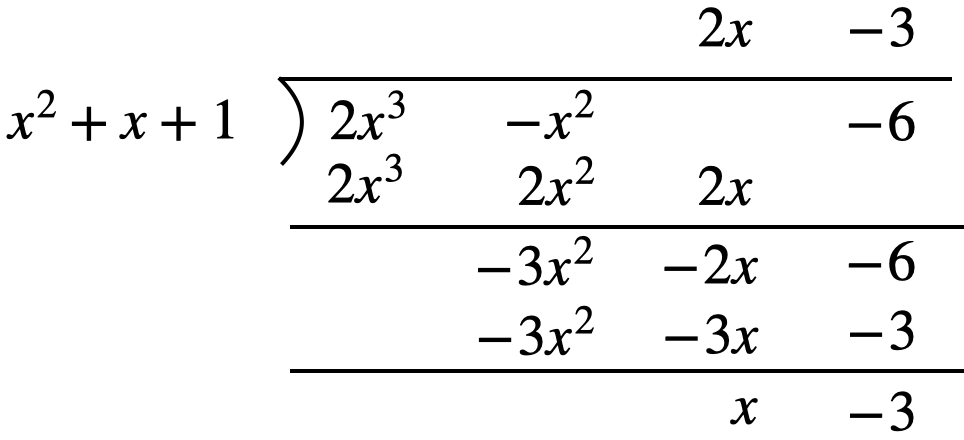
\includegraphics[width=60mm]{calculus11/poly_quot.png}
 \end{center}
\end{figure}
これより, 商は$2x-3$, 余りは$x-3$であり, 
$$
2x^3-x^2-6 = (2x-3)(x^2+x+1)+x-3. 
$$

\end{frame}



%%%%%%%%%%%%%%%%%%%%%%%%%%%%%%%%%%%%%%%%%%%%%%%%%%%%%%%%%%%%%%%%%%%%%%%%%%%%%%%%%%%%%%%
%%%%%%%%%%%%%%%%%%%%%%%%%%%%%%%%%%%%%%%%%%%%%%%%%%%%%%%%%%%%%%%%%%%%%%%%%%%%%%%%%%%%%%



\begin{frame}
\frametitle{有理関数の積分}

$\frac{1}{(x-a)^n}$の不定積分は
$$
\int \frac{dx}{(x-a)^n}=
\begin{cases}
\log|x-a| & (n=1)\\
\frac{1}{(1-n)(x-a)^{n-1}} & (n \ge 2)
\end{cases}
$$
であるから, 部分分数分解を利用して多くの有理関数の不定積分を計算することができる. 
例えば, 先の計算例より
\begin{align*}
\int \frac{x+2}{x^2(1+x)} dx
& =  \int (\frac{-1}{x}+  \frac{2}{x^2}+ \frac{1}{x+1})dx \\
& =  -\log |x| -\frac{2}{x} + \log |x+1| \\
& = \log \Big| \frac{x+1}{x}\Big| -\frac{2}{x}. 
\end{align*}


\end{frame}


%%%%%%%%%%%%%%%%%%%%%%%%%%%%%%%%%%%%%%%%%%%%%%%%%%%%%%%%%%%%%%%%%%%%%%%%%%%%%%%%%%%%%%%
%%%%%%%%%%%%%%%%%%%%%%%%%%%%%%%%%%%%%%%%%%%%%%%%%%%%%%%%%%%%%%%%%%%%%%%%%%%%%%%%%%%%%%



\begin{frame}
\frametitle{有理関数の積分}

\begin{Prob}
次の関数の不定積分を計算せよ. 
\begin{enumerate}
\item $\int \frac{1}{(x+1)(x+2)} dx$
\item $\int \frac{2x+3}{(x+1)^2} dx$
\item $\int \frac{x^3+x^2-1}{x^2-1}dx$
\end{enumerate}
\end{Prob}

\end{frame}

%%%%%%%%%%%%%%%%%%%%%%%%%%%%%%%%%%%%%%%%%%%%%%%%%%%%%%%%%%%%%%%%%%%%%%%%%%%%%%%%%%%%%%%
%%%%%%%%%%%%%%%%%%%%%%%%%%%%%%%%%%%%%%%%%%%%%%%%%%%%%%%%%%%%%%%%%%%%%%%%%%%%%%%%%%%%%%



\begin{frame}
\frametitle{有理関数の積分}

\begin{align*}
\int \frac{1}{(x+1)(x+2)} dx  = \int (\frac{1}{x+1}-\frac{1}{x+2})dx = \log\Big|\frac{x+1}{x+2}\Big|
\end{align*}

\begin{align*}
\int \frac{2x+3}{(x+1)^2} dx  = \int (\frac{2}{x+1}+\frac{1}{(x+1)^2})dx = 2\log|x+1| - \frac{1}{x+1}
\end{align*}

\begin{align*}
\int \frac{x^3+x^2-1}{x^2-1}dx & = \int (x+1 +\frac{x}{x^2-1})dx \\
& = \frac{1}{2}x^2+x+\frac{1}{2}\log|x^2-1|
\end{align*}

\end{frame}
%%%%%%%%%%%%%%%%%%%%%%%%%%%%%%%%%%%%%%%%%%%%%%%%%%%%%%%%%%%%%%%%%%%%%%%%%%%%%%%%%%%%%%%
%%%%%%%%%%%%%%%%%%%%%%%%%%%%%%%%%%%%%%%%%%%%%%%%%%%%%%%%%%%%%%%%%%%%%%%%%%%%%%%%%%%%%%





%%%%%%%%%%%%%%%%%%%%%%%%%%%%%%%%%%%%%%%%%%%%%%%%%%%%%%%%%%%%%%%%%%%%%%%%%%%%%%%%%%%%%%%
%%%%%%%%%%%%%%%%%%%%%%%%%%%%%%%%%%%%%%%%%%%%%%%%%%%%%%%%%%%%%%%%%%%%%%%%%%%%%%%%%%%%%%%




\section{今日のまとめ}
\begin{frame}
\frametitle{まとめ}   


\begin{enumerate}
\item 原始関数, 不定積分
\item 部分積分, 置換積分
\item 部分分数分解, 有理関数の積分
\end{enumerate} 

\end{frame}